\section{Trabajo de clase del lunes 7 de Octubre de 2024}

\begin{ejercicio}
    Lanzo un dado y hay 2 variables:
    \begin{align*}
        X_1 &= \left\{
        \begin{array}{cc}
            -1 & \text{impar}\\
            1 & \text{par}
        \end{array}
        \right.\\\\
        X_2 &= \left\{
        \begin{array}{ccc}
            -2 & \text{si sale} & 1,2,3\\
            0 & \text{si sale} & 4\\
            3 & \text{si sale} & 5,6
        \end{array}
        \right.\\
    \end{align*}

    Podemos calcular
    \begin{align*}
        P[X_1 = -1, X_2 = -2] &= P[\text{salga impar y salga 1,2 o 3}] = \nicefrac{2}{6}\\
        P[X_1 = -1, X_2 = 0] & = 0\\
        P[X_1 = -1, X_2 = 3] & = \nicefrac{1}{6}\\
        P[X_1 = 1, X_2 = -2] & = \nicefrac{1}{6}\\
        P[X_1 = 1, X_2 = 0] & = \nicefrac{1}{6}\\
        P[X_1 = 1, X_2 = 3] & = \underline{\nicefrac{1}{6}}\\
        & \ \ \ \ \ 1
    \end{align*}

    Podemos resumir esta información como
    \begin{center}
        \begin{tabular}{c | c c c | c }
            \scriptsize{$X_1 \backslash X_2$} & -2 & 0 & 3 &\phantom{\scriptsize{$X_1 \backslash X_2$}}\\
            \hline
            -1 & \nicefrac{2}{6} & 0 & \nicefrac{1}{6}&\\
            1 & \nicefrac{1}{6} & \nicefrac{1}{6} & \nicefrac{1}{6}&\\
            \hline
            &&&&\\
        \end{tabular}
    \end{center}
    Sabeos que  
    \begin{gather*}
        P_{X_1, X_2}(x_1, x_2) = P[X_1 \leq x_1 , X_2 \leq x_2]
    \end{gather*}
    Por lo que
    \begin{center}
        \begin{tabular}{ccccc}
            0 & si & $x_1\leq -1$ & o & $x_2 \leq -2$\\
            \nicefrac{2}{6} & si & $-1 \leq x_1< 1 $ & y & $-2 \leq x_2 < 3$\\
            \nicefrac{2}{6} & si & $-1 \leq x_1< 1 $ & y & $x_2 \geq 3$\\
            \nicefrac{3}{6} & si & $ x_1 \geq 1$ & y & $-2 \leq x_2 < 0$\\
            \nicefrac{4}{6} & si & $ x_1 \geq 1$ & y & $0 \leq x_2 < 3$\\
            1 & si & $ x_1 \geq 1$ & y & $x_2 \geq 3$\\
        \end{tabular}
    \end{center}

    \begin{center}
        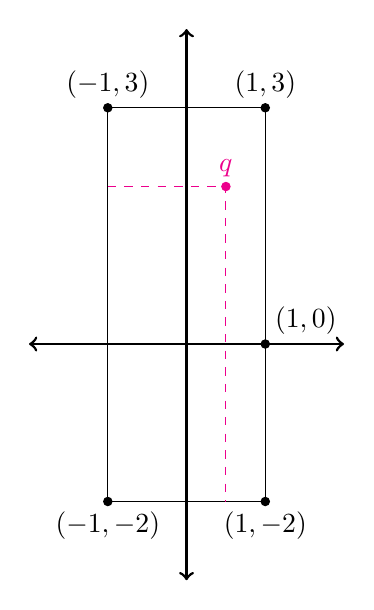
\begin{tikzpicture}
            % Desactiva los caracteres conflictivos
            \shorthandoff{>} % Para poner puntas de flecha

            \draw[line width=1pt, <->] (0, -3) -- (0,4);
            \draw[line width=1pt, <->] (-2, 0) -- (2,0);

            \filldraw (-1,3) circle (1.5pt)  node[above] {$(-1,3)$};
            \filldraw (1,3) circle (1.5pt)  node[above] {$(1,3)$};
            \filldraw (-1,-2) circle (1.5pt)  node[below] {$(-1,-2)$};
            \filldraw (1,-2) circle (1.5pt)  node[below] {$(1,-2)$};
            \filldraw (1,0) circle (1.5pt)  node[anchor=south west] {$(1,0)$};

            \draw (-1,3) -- (1,3) -- (1,-2) -- (-1,-2)-- (-1,3);

            \draw[magenta, dashed] (-1,2) -- (0.5, 2) -- (0.5, -2);
            \filldraw[magenta] (0.5,2) circle (1.5pt)  node[above] {$q$};
        \end{tikzpicture}
    \end{center}

    \begin{gather*}
        P[X_1+X_2 \leq 1] = P[X\in \{(-1,-2), (-1,0), (1, -2), (1,0)\}] = \nicefrac{2}{6} + 0 + \nicefrac{1}{6} + \nicefrac{1}{6} = \nicefrac{2}{3}
    \end{gather*}
    
\end{ejercicio}
\hspace{0.5cm}
\begin{ejemplo}
    Dos vectores aleatorios dimensionales $X=(X_1, X_2)$ y $\eps = (\eps_1, \eps_1) \in \bb{R}^2_+$
    \begin{gather*}
        F_{\underline{X}}(X_1 + \eps_1, X_2+\eps_2) - F_{\underline{X}}(X_1, X_2+\eps_2) - F_{\underline{X}}(X_1 + \eps_1, X_2) + F_{\underline{X}}(X_1, X_2) \geq 0
    \end{gather*}
    Demostrar que no es una función de distribución (probar con la propiedad 4).
\end{ejemplo}
